\documentclass[tikz]{standalone}
%\usepackage{tikz}
\usetikzlibrary{positioning, backgrounds,fit,shapes.geometric}

\usepackage{xcolor}
\definecolor{position-color}{HTML}{F3EACE}
\definecolor{direction-color}{HTML}{E7F8E8}

\begin{document}
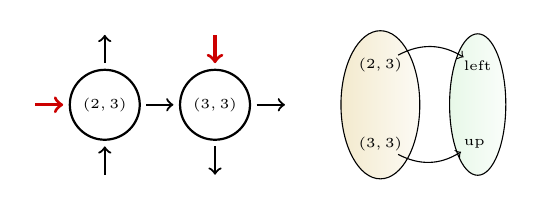
\begin{tikzpicture}

\begin{scope}[every node/.style={circle, draw, minimum size=0.2cm,}, shorten >=2pt, shorten <=2pt, thick]

\node(n1) at (2,3) {\tiny $(2,3)$};
\node(n2) at (3.4,3) {\tiny $(3,3)$};

\draw[->] (n1.north) -- ++ (0, 0.5);
\draw[->] (n1.east)  -- (n2.west);
\draw[<-] (n1.south) -- ++ (0,-0.5);
\draw[<-,very thick, red!80!black] (n1.west)  -- ++ (-0.5,0);

\draw[<-,very thick, red!80!black] (n2.north) -- ++(0,0.5);
\draw[->] (n2.east)  -- ++(0.5,0);
\draw[->] (n2.south) -- ++(0,-0.5);
\end{scope}

\begin{scope}[xshift=5.5cm, yshift=3cm, every node/.style={inner sep=1pt}, node distance=0.7cm]
\node(n1) at(0,0.5) {\tiny $(2,3)$};
\node(n2) at(0,-0.5){\tiny $(3,3)$};

\node(t1) [right=of n1]{\tiny left};
\node(t2) [right=of n2]{\tiny up};

\draw[->] (n1) to[bend left]  (t1);
\draw[->] (n2) to[bend right] (t2);


\begin{scope}[on background layer,
border/.style={draw, ellipse, left color=#1, right color=#1!20!white}
]
\node[border=position-color, fit=(n1)(n2)]{};
\node[border=direction-color, fit=(t1)(t2)]{};
\end{scope}

\end{scope}
 
\end{tikzpicture}
\end{document}
